\chapter{Part 4f: Instruction Level Parallelism (ILP) Besides and Beyond Superscalars}

Instruction-Level Parallelism (ILP) is the measure of how many operations in a computer program can be performed simultaneously. The goal of ILP is to exploit parallel execution within a single thread to improve performance. Traditional \emph{superscalar} architectures achieve ILP by issuing multiple instructions in one clock cycle, but new challenges arise when hardware and program behavior limit the amount of parallelism that can be extracted.

\section{Superscalar Execution}
Modern high-performance processors often implement \emph{superscalar} execution, where multiple instructions are issued (i.e., started) in the same clock cycle to increase throughput. However, to realize sustained parallelism, several requirements must be met:

\begin{center}
    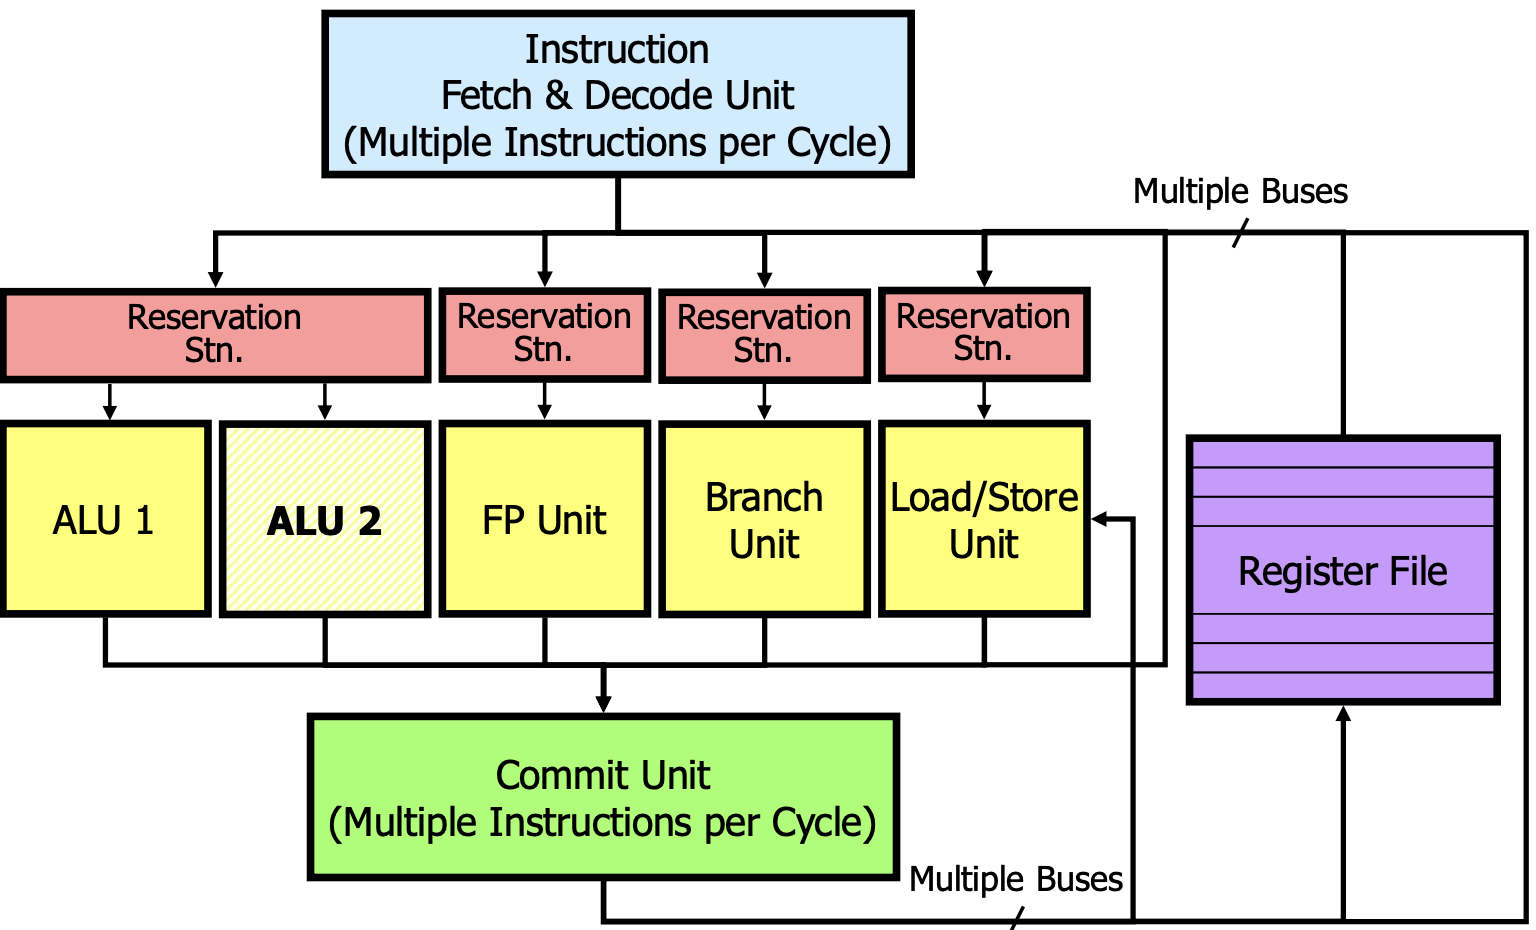
\includegraphics[width=0.45\textwidth]{chapters/chapter4f/images/superscalar.png}
\end{center}

\begin{itemize}
  \item \textbf{Fetch more instructions per cycle.}\\
  An instruction cache with sufficient bandwidth is needed to supply multiple instructions each cycle. Without adequate fetch capacity, the pipeline stalls and cannot exploit superscalar capabilities.

  \item \textbf{Commit more instructions per cycle.}\\
  To retire (commit) multiple instructions per cycle, the \emph{reorder buffer} (ROB) and the \emph{register file} must have enough ports and resources. A lack of commit bandwidth creates a bottleneck, undoing the benefits of parallel execution in earlier stages.

  \item \textbf{Obey data and control dependencies.}\\
  Even if hardware can fetch and commit multiple instructions per cycle, \emph{data hazards} and \emph{control hazards} must be respected. Modern superscalar designs typically use out-of-order (dynamic) scheduling to track dependencies and reorder instructions for higher throughput while maintaining correctness.
\end{itemize}

Despite advanced hardware techniques, data and control hazards impose fundamental limits on how much ILP can be extracted. In practice, balancing fetch, execute, and commit bandwidth with careful hazard management remains the central challenge of superscalar execution.

\section{Dealing with Control Hazards}
Superscalar processors can issue multiple instructions each cycle, but they are especially sensitive to branching instructions that disrupt the flow of fetched instructions. This section outlines several techniques that help mitigate the performance penalties of branches.

\subsection{Dynamic Branch Prediction}
\label{sec:branch-pred}
Branches create uncertainty: the processor needs to know which instruction addresses to fetch next. Two main problems arise when exploiting ILP:
\begin{itemize}
    \item \textbf{True data dependencies}, which are unavoidable since some instructions inherently depend on the results of others.
    \item \textbf{Branches}, which determine \emph{where} to look for further instructions.
\end{itemize}

\noindent
\textbf{Static Prediction}\\
Early branch prediction methods (e.g., always-taken, never-taken, or simple compiler hints) often fail to anticipate dynamic behavior accurately because they cannot adapt to runtime conditions.

\noindent
\textbf{Dynamic Prediction}\\
Dynamic branch prediction learns from past behavior. By using hardware structures that track how often a branch was taken, the predictor can adapt and refine its guesses over time, increasing overall accuracy and reducing wasted work from mispredicted branches.

\subsection{Branch History Table (BHT)}
A key component in many dynamic branch predictors is the \emph{Branch History Table (BHT)}, which uses part of the \textit{Program Counter} (PC) as an index. Each BHT entry stores one or more bits that represent the likelihood of a branch being taken or not taken.

\begin{center}
    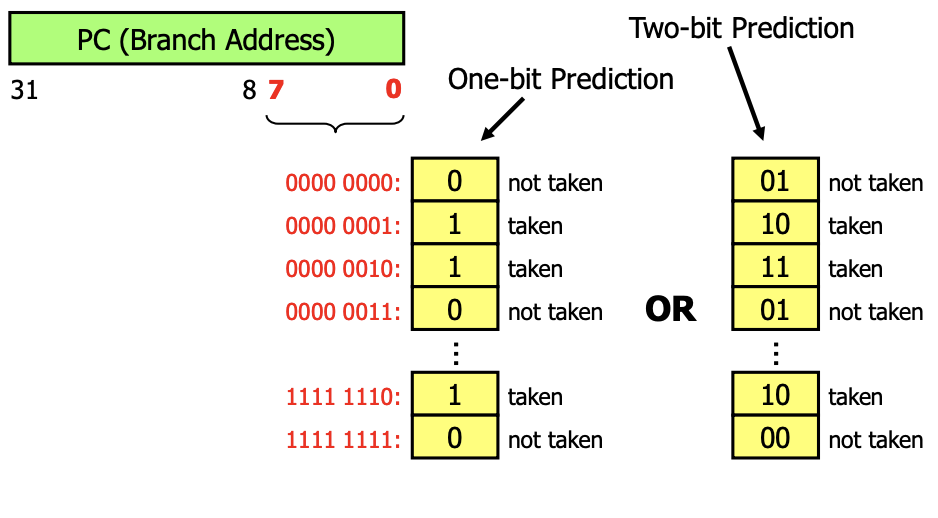
\includegraphics[width=0.45\textwidth]{chapters/chapter4f/images/bht.png}
\end{center}

\begin{itemize}
    \item \textbf{Address Indexing:} The lower bits of the PC (e.g., bits 7:0) index into the BHT.
    \item \textbf{Prediction Storage:}
    \begin{itemize}
        \item \emph{One-bit Prediction:} Each entry stores a single bit:
              \begin{itemize}
                \item \texttt{0}: Not taken
                \item \texttt{1}: Taken
              \end{itemize}
        \item \emph{Two-bit Prediction:} Each entry stores two bits:
              \begin{itemize}
                \item \texttt{00}: Strongly not taken
                \item \texttt{01}: Weakly not taken
                \item \texttt{10}: Weakly taken
                \item \texttt{11}: Strongly taken
              \end{itemize}
    \end{itemize}
    \item \textbf{Update Mechanism:} Predictions are updated based on whether the branch was actually taken, helping the hardware adapt to program behavior.
\end{itemize}

\subsection{Speculative Execution}
Speculative execution is a performance optimization that issues and executes instructions \emph{before} a branch outcome is resolved. This reduces pipeline bubbles that occur when the processor must otherwise wait.

\begin{itemize}
  \item \textbf{Dynamic Branch Prediction:} The processor fetches and decodes along the predicted path, using minimal resources so that incorrect speculations are easily discarded.
  \item \textbf{Results Handling:} Computed results remain \emph{uncommitted} until the branch outcome is confirmed.
  \item \textbf{Recovery:} If a misprediction occurs, the processor \emph{squashes} any partially executed instructions from the wrong path and resumes from the correct path.
\end{itemize}

\subsection{Branches in the Reorder Buffer}
Modern out-of-order processors track branch instructions and their outcomes in a \emph{Reorder Buffer (ROB)}. Because branches are speculative, the ROB must handle both correct and incorrect predictions gracefully.

\begin{center}
    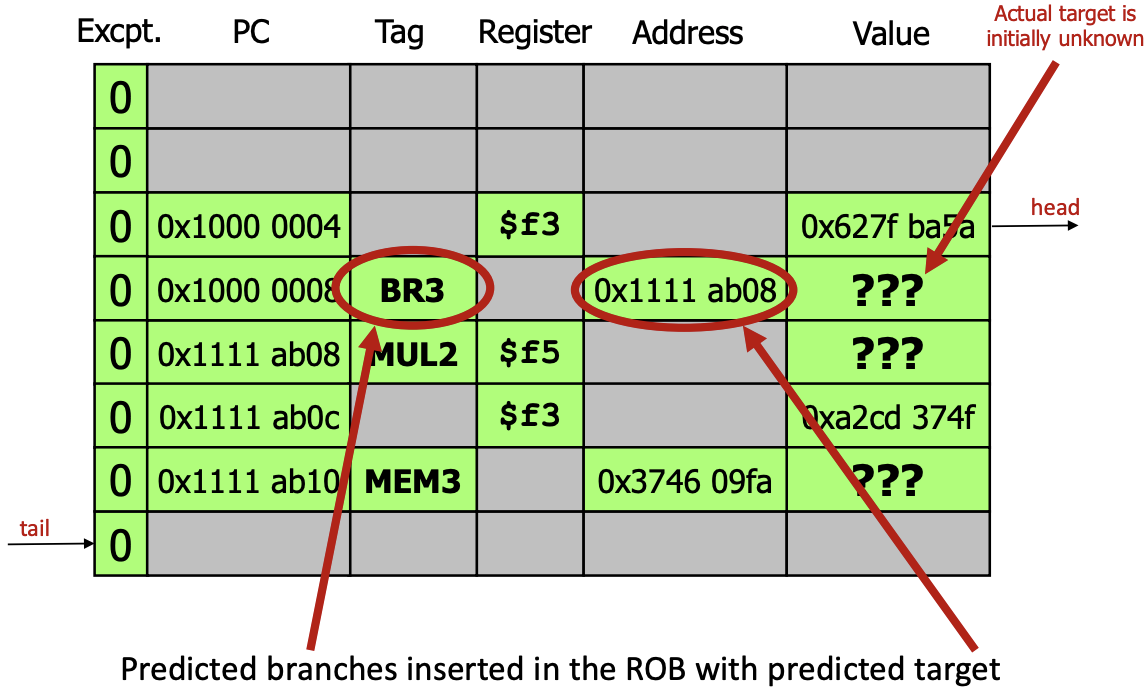
\includegraphics[width=0.45\textwidth]{chapters/chapter4f/images/rob.png}
\end{center}

\begin{itemize}
    \item \textbf{Correctly Predicted Branches:}
    When the actual branch target matches the prediction, the branch instruction is marked \emph{resolved} and can be retired normally.
    \item \textbf{Mispredicted Branches:}
    If the actual branch target differs from the prediction, all instructions following that branch in the ROB are invalidated (\emph{squashed}), and fetch restarts from the correct target address.
\end{itemize}

These mechanisms ensure the processor can continue running instructions \emph{speculatively}, reaping the benefits of ILP while safeguarding correctness.

\section{Beyond Superscalars: Simultaneous Multithreading (SMT)}
When a superscalar pipeline is unable to find sufficient parallelism within a single thread, an alternative is to keep the hardware busy by issuing instructions from multiple threads. \emph{Simultaneous Multithreading (SMT)} does exactly this, allowing multiple independent threads to utilize the same execution resources in parallel.

\begin{center}
    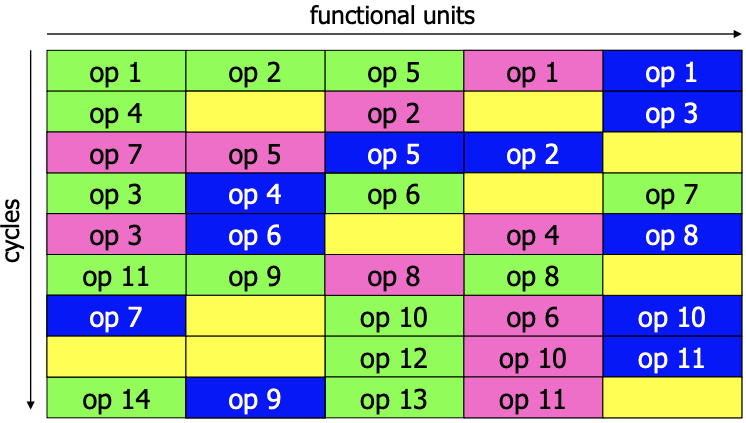
\includegraphics[width=0.45\textwidth]{chapters/chapter4f/images/smt.png}
\end{center}

\subsection*{SMT vs.\ Single-Thread Superscalar}
A dynamically scheduled superscalar typically manages only one thread at a time. It has:
\begin{itemize}
  \item A single set of \emph{reservation stations} to track operand availability.
  \item One \emph{reorder buffer} to handle out-of-order execution and in-order retirement.
\end{itemize}

\subsection*{Adding SMT Support}
An SMT processor can simultaneously issue instructions from multiple threads in the same cycle:
\begin{itemize}
  \item \textbf{Multiple PCs:} Each hardware thread needs its own program counter.
  \item \textbf{Extended Register File:} Either a separate set of registers per thread or a unified file with thread IDs.
  \item \textbf{Multiple or Extended ROBs:} Each thread must track and retire its instructions in order; thread IDs are often added to each entry.
\end{itemize}

\begin{center}
    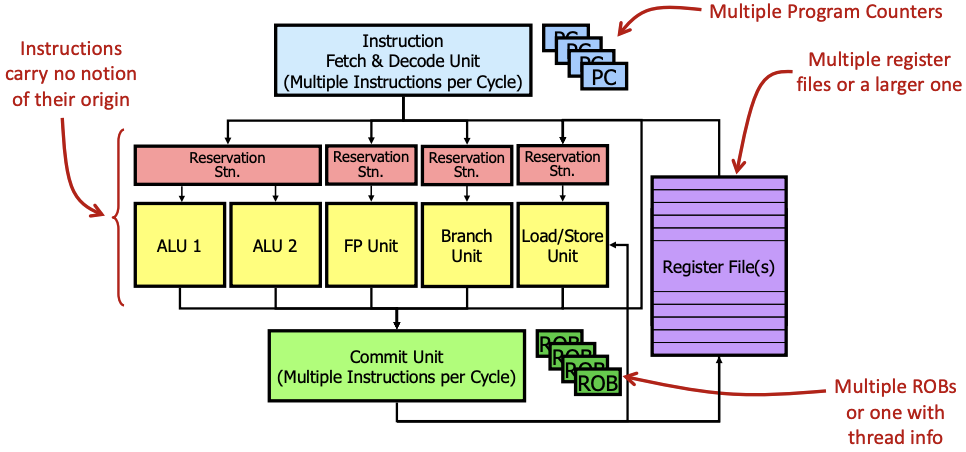
\includegraphics[width=0.55\textwidth]{chapters/chapter4f/images/smt_proc.png}
\end{center}

Because thread instructions share the same functional units, SMT can achieve higher resource utilization, especially when one thread stalls or has limited ILP on its own. However, hardware becomes more complex, and caches and other shared structures must be carefully managed.

\section{Memory Considerations: Nonblocking Caches}
Even with a highly parallel core, performance may be bottlenecked by slow memory operations. If a load instruction misses in the cache, superscalar and SMT designs benefit from continuing other work rather than stalling immediately. \emph{Nonblocking caches} help achieve this.

\subsection*{Example of Memory Stall}
\begin{assembly}
lw   $t2, 0($t0)    # t2 = mem[t0]
lw   $t3, 0($t1)    # t3 = mem[t1]
addi $t3, $t3, 123
andi $t3, $t3, 0xff
\end{assembly}
If the first load (\texttt{lw $t2, 0($t0)}) results in a cache miss, a simple blocking cache would stall the pipeline until the data returns from memory. However, a \emph{nonblocking cache} lets subsequent instructions continue if they do not depend on the missing data.

\subsection*{Hit Under Miss and Miss Under Miss}
\begin{itemize}
  \item \textbf{Hit Under Miss:} Serves new cache requests from different addresses while a miss is being resolved.
  \item \textbf{Miss Under Miss:} Handles multiple outstanding misses, overlapping latencies from the memory system.
\end{itemize}

These mechanisms greatly improve throughput by allowing the processor to exploit ILP (and multiple threads in SMT) while memory requests are pending.

\newpage
\section{VLIW: Very Long Instruction Word Architecture}

VLIW (Very Long Instruction Word) architecture exploits \emph{instruction-level parallelism} (ILP) by bundling multiple operations into a single long instruction word. Unlike pipelined processors, which execute instructions sequentially (albeit overlapped in time), VLIW delegates the responsibility of scheduling parallel operations to the compiler. The compiler groups independent operations that can be executed simultaneously into fixed-width instruction bundles.
\begin{center}
    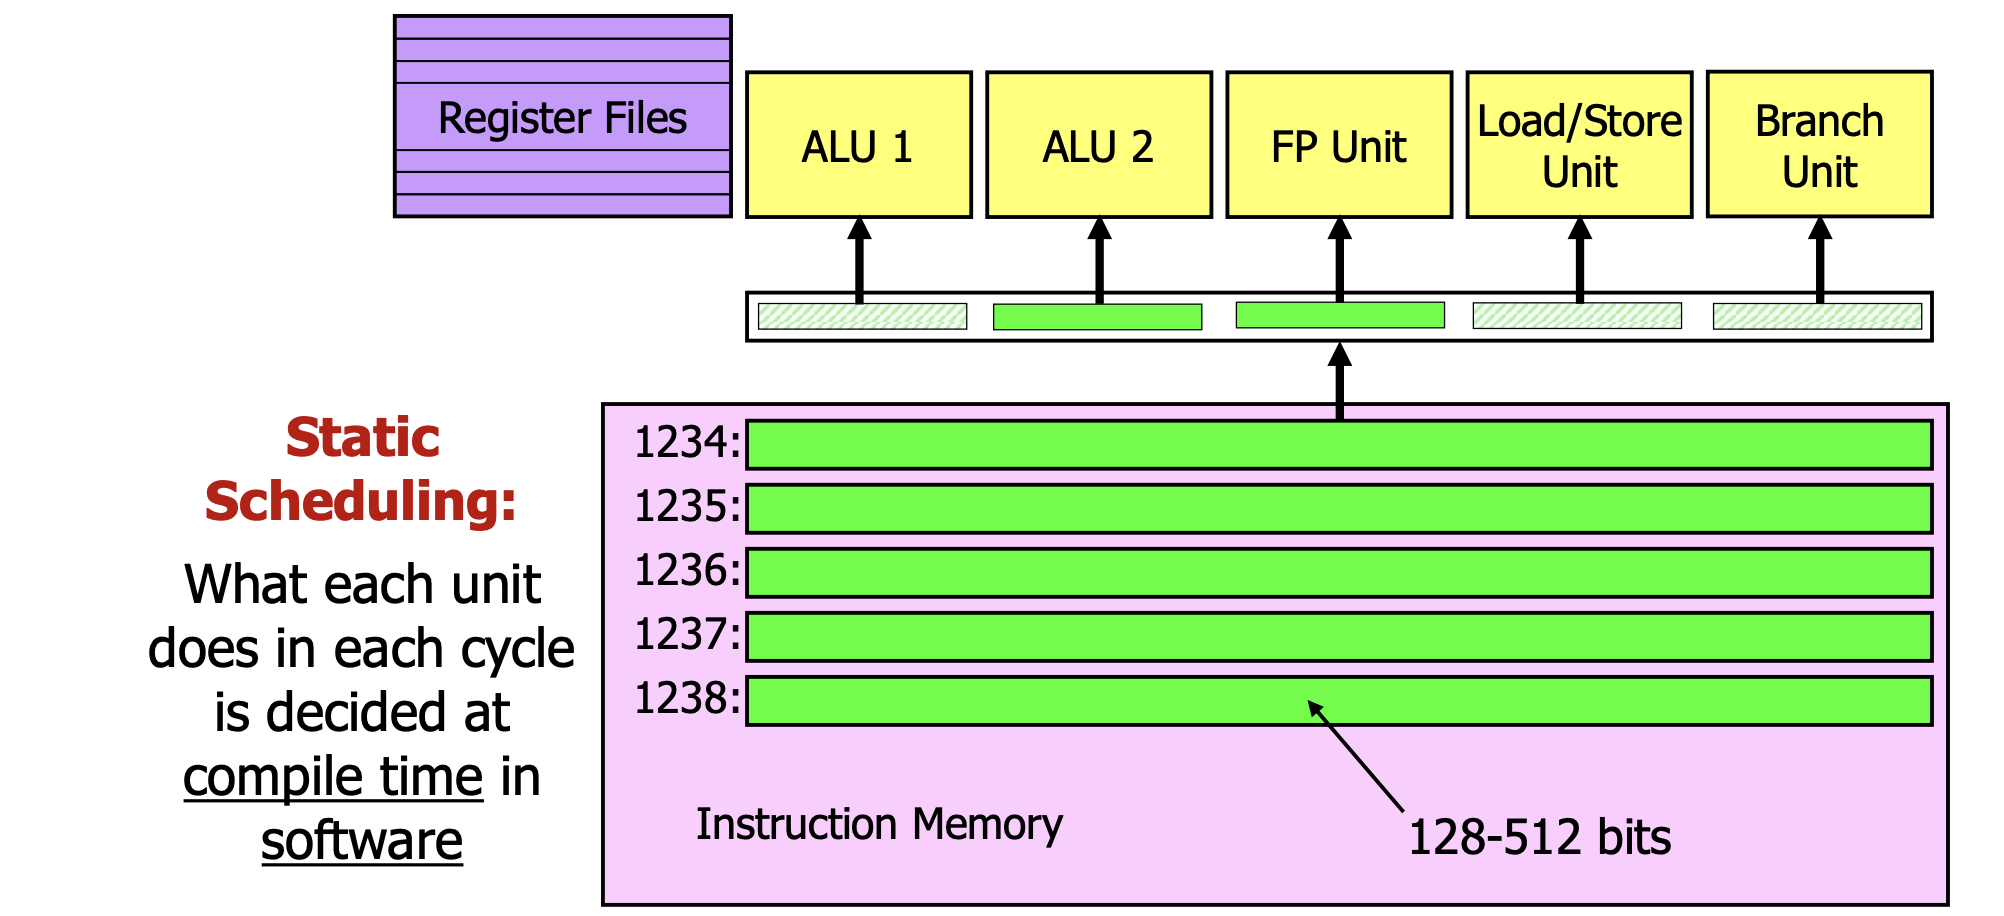
\includegraphics[width=0.65\textwidth]{chapters/chapter4f/images/VLIW.png}
\end{center}
\subsection{Core Concepts}
\begin{itemize}
    \item \textbf{Fixed Instruction Format:} Each instruction consists of multiple slots, where each slot is assigned to a specific functional unit (e.g., arithmetic logic unit (ALU), memory unit).
    \item \textbf{Static Scheduling:} The compiler analyzes dependencies in the code and schedules instructions into bundles. Dynamic dependency checks and scheduling hardware are not needed.
    \item \textbf{Compiler-Driven:} The compiler must ensure that operations within one bundle are independent (or safe) to execute in parallel.
\end{itemize}

\subsection{Example: VLIW vs. Pipelined Execution}

Consider the following simple code fragment in a C-like pseudocode:
\begin{verbatim}
a = b + c;   // Operation 1
d = e - f;   // Operation 2
g = h * i;   // Operation 3
x = arr[j];  // Operation 4 (memory load)
\end{verbatim}

\subsubsection*{Pipelined Processor Execution}
In a pipelined processor, these instructions may be overlapped in execution stages (fetch, decode, execute, etc.). However, they are still issued one after another. For example:
\begin{enumerate}
    \item \textbf{Cycle 1:} Fetch Operation 1
    \item \textbf{Cycle 2:} Decode Operation 1, Fetch Operation 2
    \item \textbf{Cycle 3:} Execute Operation 1, Decode Operation 2, Fetch Operation 3
    \item \textbf{Cycle 4:} Execute Operation 2, Decode Operation 3, Fetch Operation 4
    \item \textbf{Cycle 5:} Execute Operation 3, Execute Operation 4
\end{enumerate}
The pipeline overlaps different stages of separate instructions but does not execute multiple operations simultaneously in the same cycle.

\subsubsection*{VLIW Processor Execution}
Assume a simple VLIW processor with 3 functional units:
\begin{itemize}
    \item ALU1: Arithmetic operations.
    \item ALU2: Arithmetic operations.
    \item MEM: Memory load/store operations.
\end{itemize}

The VLIW compiler analyzes dependencies and groups independent operations into a single long instruction. Given the code, the compiler may schedule as follows:

\paragraph{VLIW Instruction Format:}
\[
\texttt{| ALU1 \quad|\quad ALU2 \quad|\quad MEM |}
\]

\paragraph{Scheduled VLIW Instructions:}
\begin{enumerate}
    \item \textbf{Cycle 1:}
    \begin{itemize}
        \item \texttt{ALU1:} \texttt{ADD r1, r2, r3} \quad (compute \texttt{a = b + c})
        \item \texttt{ALU2:} \texttt{SUB r4, r5, r6} \quad (compute \texttt{d = e - f})
        \item \texttt{MEM:} \texttt{LOAD r7, [arr + r8]} \quad (perform memory load for \texttt{x = arr[j]})
    \end{itemize}
    \item \textbf{Cycle 2:}
    \begin{itemize}
        \item \texttt{ALU1:} \texttt{MUL r9, r10, r11} \quad (compute \texttt{g = h * i})
        \item \texttt{ALU2:} \texttt{NOP} \quad (no operation)
        \item \texttt{MEM:} \texttt{NOP} \quad (no operation)
    \end{itemize}
\end{enumerate}

\subsubsection*{Key Differences}
\begin{itemize}
    \item \textbf{Instruction Issue:}
    \begin{itemize}
        \item \emph{Pipelined:} Issues one instruction per cycle and overlaps the stages.
        \item \emph{VLIW:} Issues a bundle of operations in one cycle, executing them concurrently.
    \end{itemize}
    \item \textbf{Scheduling:}
    \begin{itemize}
        \item \emph{Pipelined:} Hardware manages instruction overlapping.
        \item \emph{VLIW:} The compiler statically schedules independent instructions into a single, long instruction word.
    \end{itemize}
\end{itemize}

\subsection{Summary}
VLIW architectures shift complexity from hardware to the compiler, allowing multiple operations to execute in parallel within a single clock cycle. This enables efficient exploitation of ILP but requires careful compile-time analysis to ensure that parallel execution is both possible and correct.

